\chapter[Creating The Polar NRZ Ensemble]{Creating The Polar NRZ Ensemble}
\label{cp:creating-the-polar-nrz-ensemble}

Similar to what we did in the previous chapter when we were creating the
unipolar ensemble, we will apply the same steps to create the polar NRZ
ensemble.
\begin{listing} [!htpb]
    \caption{Creating the Polar NRZ Ensemble.}
    \label{listing:Polar-Ensemble}
    \begin{minted}{matlab}
%% Polar NRZ
fprintf('\nPolar NRZ\n');
pulse_polar_NRZ = ones(1, L);
ylim_polar_NRZ  = [-A-1, A+1];
color_polar_NRZ = [0 0.4470 0.7410];

ensample_polar_NRZ = build_ensemble(data, A, pulse_polar_NRZ, N_realizations, L, 'polar');
    \end{minted}
\end{listing}

\begin{figure}[!htpb]
    \centering
    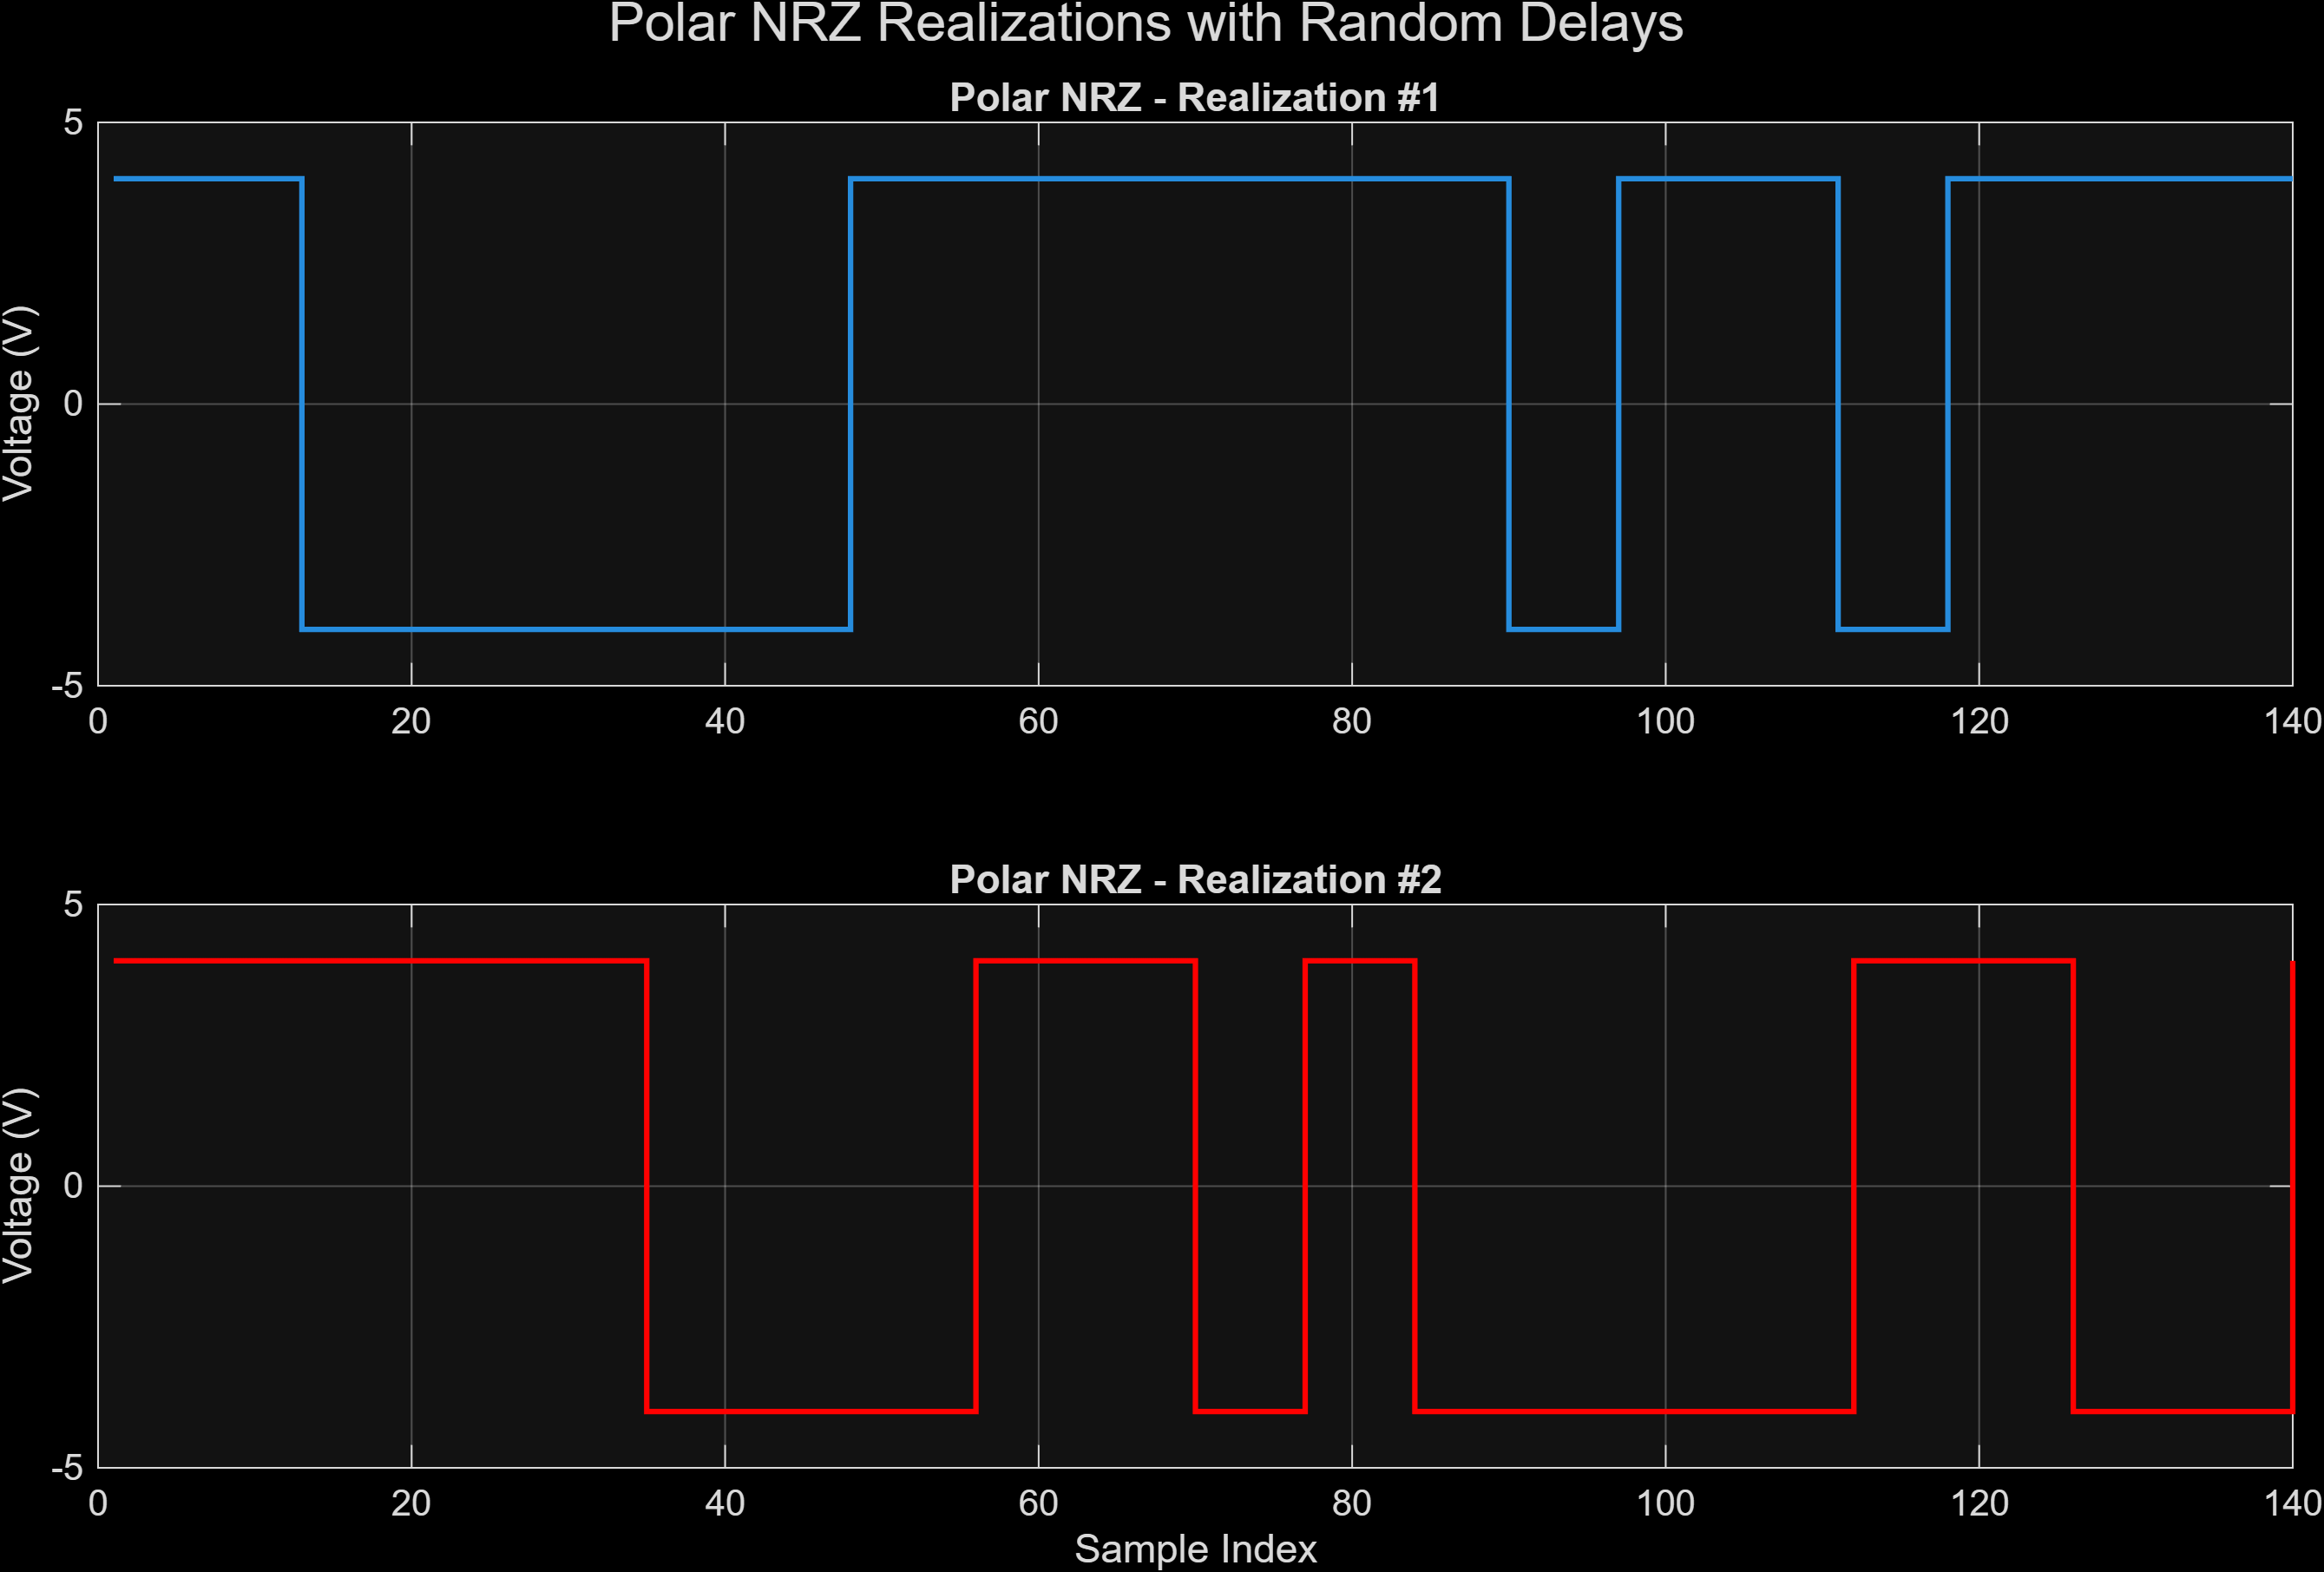
\includegraphics[width=0.75\linewidth]{Figures/Polar_NRZ_-_Realization_2.png}
    \caption[Realization 1 and Realzation 2 from the Polar Ensemble]{Realization 1 and Realzation 2 from the Polar Ensemble.}
    \label{fig:POLAR-ENSEMBLE}
\end{figure}

As we can see in \autoref{fig:POLAR-ENSEMBLE}
\begin{itemize}
    \item The signal is either at $-A$ or at $+A$, which is the expected behavior for the
          polar NRZ line code.
    \item The pulse shape is rectangular, with a duration of $L$ samples per bit.
\end{itemize}
